\documentclass[hidelinks,12pt,dvipsnames,border=2pt]{standalone}
%\usepackage[top=0.7in, bottom=0.8in, left=1in, right=1in]{geometry}
\usepackage{tikz}
\usepackage{hyperref}
\usetikzlibrary{arrows}
\usetikzlibrary{shapes}
\usepackage{enumitem}
\usepackage{bm}
\usepackage{mathdots}
\usepackage{amsmath}
\usepackage{tcolorbox}
\usetikzlibrary{shadings}
\usetikzlibrary{decorations.pathreplacing}
\usepackage{helvet}
\usepackage{url}
\usepackage{graphicx}
\usetikzlibrary{arrows.meta,positioning,fit,calc}
\renewcommand{\familydefault}{\sfdefault}

\definecolor{p1}{HTML}{440154}
\definecolor{p2}{HTML}{414487}
\definecolor{p3}{HTML}{2A788E}
\definecolor{p4}{HTML}{22A884}
\definecolor{p5}{HTML}{7AD151}
\definecolor{p6}{HTML}{21908C}
\definecolor{p7}{HTML}{22A884}
\definecolor{p8}{HTML}{43BF71}
\definecolor{p9}{HTML}{7AD151}
\usetikzlibrary{arrows,decorations.pathmorphing,backgrounds,fit,positioning,shapes.symbols,chains}

\begin{document}
	
% trim=left botm right top
\begin{tikzpicture}

\node at (0,0) {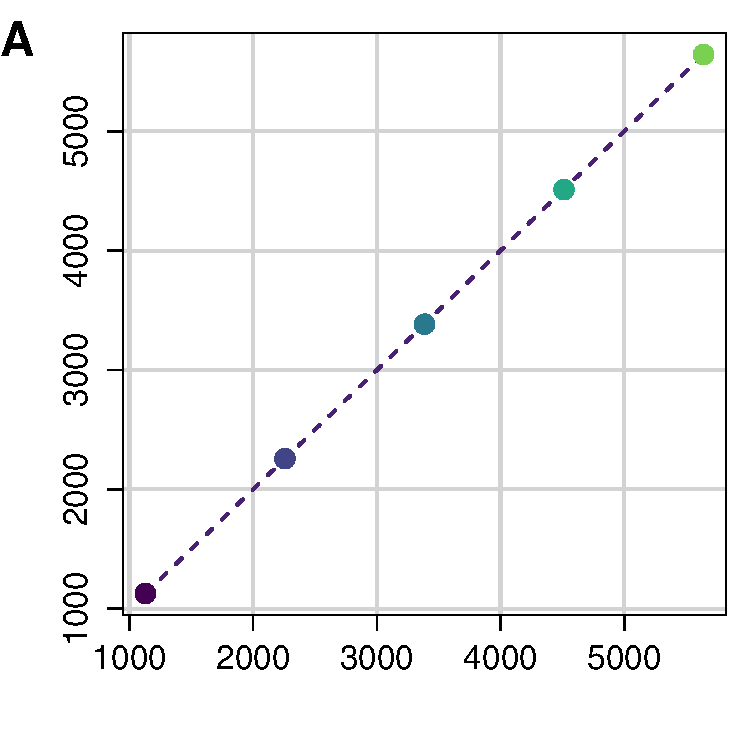
\includegraphics[width=\textwidth]{standard_normal_manhattan_sample-mean_vs_theoretical-mean3.pdf}};
\node at (13.75,0) {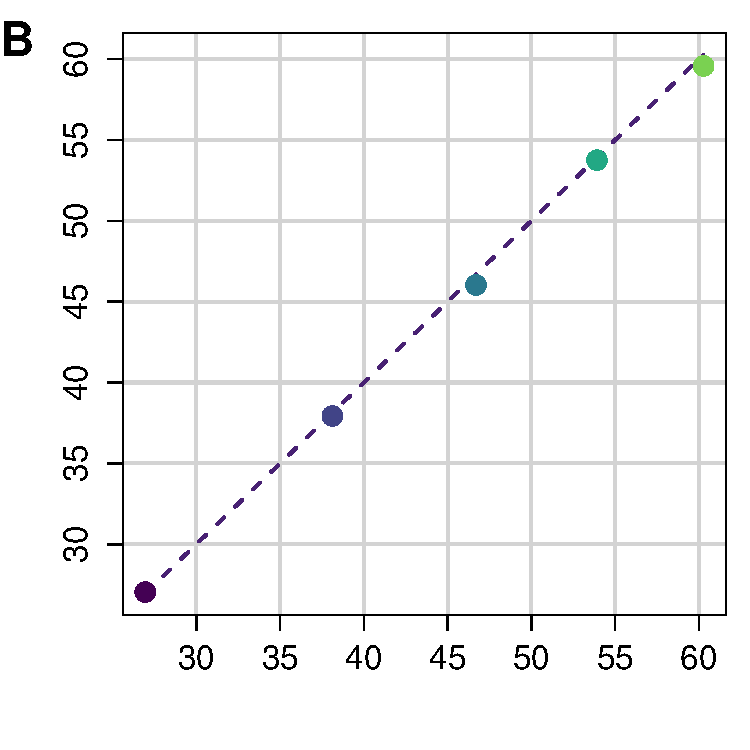
\includegraphics[width=\textwidth]{standard_normal_manhattan_sample-SD_vs_theoretical-SD3.pdf}};

\node[rotate=90,xscale=1.9,yscale=1.9] at (-6.6,0.8) {Theoretical Mean};
\node[xscale=1.9,yscale=1.9] at (0.9,-6.3) {Simulated Mean};

\node[rotate=90,xscale=1.9,yscale=1.9] at (7.15,0.8) {Theoretical SD};
\node[xscale=1.9,yscale=1.9] at (14.65,-6.3) {Simulated SD};

%\node[rotate=90,xscale=1.9,yscale=1.9] at (-6.5,-11.6) {Distance (Mean $\pm$ SD)};

%\node[rotate=90,xscale=2.1,yscale=2.1] at (-7.5,-5.1) {Distance (Mean $\pm$ SD)};

%\node[xscale=1.9,yscale=1.9] at (7.95,-6.3) {Number of Attributes ($p$)};

\node[xscale=1.9,yscale=1.9] at (7.95,9) {Moments of Manhattan Distances in Standard Normal Data};

\node[xscale=2.4,yscale=2.4] at (3.95,7.8) {\textcolor{p1}{$\bullet$}};
\node[xscale=2.4,yscale=2.4] at (6.2,7.8) {\textcolor{p2}{$\bullet$}};
\node[xscale=2.4,yscale=2.4] at (8.45,7.8) {\textcolor{p3}{$\bullet$}};
\node[xscale=2.4,yscale=2.4] at (10.7,7.8) {\textcolor{p4}{$\bullet$}};
\node[xscale=2.4,yscale=2.4] at (12.95,7.8) {\textcolor{p5}{$\bullet$}};
\node[xscale=1.5,yscale=1.5] at (2.45,7.1) {p =};
\node[xscale=1.5,yscale=1.5] at (3.95,7.2) {1000};
\node[xscale=1.5,yscale=1.5] at (6.2,7.2) {2000};
\node[xscale=1.5,yscale=1.5] at (8.45,7.2) {3000};
\node[xscale=1.5,yscale=1.5] at (10.7,7.2) {4000};
\node[xscale=1.5,yscale=1.5] at (12.95,7.2) {5000};
\node[draw,line width=0.3mm,text width=12cm,text height=1.1cm] at (7.84,7.5) {};

%\node[xscale=1.65,yscale=1.65] at (21.3,3.8) {\textcolor{p2}{$\bullet$}};
%\node[xscale=1.65,yscale=1.65] at (23.2,3.8) {$p=1500$};

%\node[xscale=1.65,yscale=1.65] at (21.3,3.1) {\textcolor{p3}{$\bullet$}};
%\node[xscale=1.65,yscale=1.65] at (23.2,3.1) {$p=2000$};

%\node[xscale=1.65,yscale=1.65] at (21.3,2.4) {\textcolor{p4}{$\bullet$}};
%\node[xscale=1.65,yscale=1.65] at (23.2,2.4) {$p=2500$};

%\node[xscale=1.65,yscale=1.65] at (21.3,1.7) {\textcolor{p5}{$\bullet$}};
%\node[xscale=1.65,yscale=1.65] at (23.2,1.7) {$p=3000$};

%\node[xscale=1.65,yscale=1.65] at (21.3,1) {\textcolor{p6}{$\bullet$}};
%\node[xscale=1.65,yscale=1.65] at (23.2,1) {$p=3500$};

%\node[xscale=1.65,yscale=1.65] at (21.3,0.3) {\textcolor{p7}{$\bullet$}};
%\node[xscale=1.65,yscale=1.65] at (23.2,0.3) {$p=4000$};

%\node[xscale=1.65,yscale=1.65] at (21.3,-0.4) {\textcolor{p8}{$\bullet$}};
%\node[xscale=1.65,yscale=1.65] at (23.2,-0.4) {$p=4500$};

%\node[xscale=1.65,yscale=1.65] at (21.3,-1.1) {\textcolor{p9}{$\bullet$}};
%\node[xscale=1.65,yscale=1.65] at (23.2,-1.1) {$p=5000$};

%\node[draw,line width=0.3mm,text width=4cm,text height=7.6cm] at (22.8,2.31) {};

%\node[xscale=1.65,yscale=1.65] at (22.8,5.6) {\# Attributes};

\end{tikzpicture}

\end{document}